\documentclass[aspectratio=43]{beamer}
% \documentclass[aspectratio=169]{beamer}

% Title --------------------------------------------
\title[Lecture 2: Elements of quantitative research]{\Large Elements of quantitative research}
\author[]{Francisco Villamil}
\date[]{Research Design for Social Sciences\\MA Computational Social Science, UC3M\\Fall 2023}

%%% NOTE -- CHECK THIS: https://github.com/paulgp/beamer-tips


%%% Building heavily on https://github.com/kylebutts/templates

% xcolor, define them
\usepackage{xcolor}

% TEXT COLORS
\definecolor{red}{HTML}{9a2515}
\definecolor{yellow}{HTML}{EBC944}
\definecolor{asher}{HTML}{555F61}
\definecolor{jet}{HTML}{131516}

% THEME COLORS
\definecolor{accent}{HTML}{107895}
\definecolor{accent2}{HTML}{9a2515}

% Color commands
\newcommand\red[1]{{\color{red}#1}}
\newcommand\yellow[1]{{\color{yellow}#1}}
\newcommand\asher[1]{{\color{asher}#1}}

\newcommand\BGred[1]{{\colorbox{red!80!white}{#1}}}
\newcommand\BGyellow[1]{{\colorbox{yellow!80!white}{#1}}}
\newcommand\BGasher[1]{{\colorbox{asher!80!white}{#1}}}

% Appendix numbering
\usepackage{appendixnumberbeamer}

% Beamer Options -------------------------------------

% Background
\setbeamercolor{background canvas}{bg = white}

% Change text margins
\setbeamersize{text margin left = 25pt, text margin right = 15pt}

% \alert
\setbeamercolor{alerted text}{fg = accent2}

% Frame title
\setbeamercolor{frametitle}{bg = white, fg = jet}
\setbeamercolor{framesubtitle}{bg = white, fg = accent}
\setbeamerfont{framesubtitle}{size = \small, shape = \itshape}

% Block
\setbeamercolor{block title}{fg = white, bg = accent2}
\setbeamercolor{block body}{fg = jet, bg = jet!10!white}

% Title page
\setbeamercolor{title}{fg = jet}
\setbeamercolor{subtitle}{fg = accent}

%% Custom \maketitle and \titlepage
\setbeamertemplate{title page}
{
    \begin{centering}
      % \vspace{20mm}
      {\Large \usebeamerfont{title}\usebeamercolor[fg]{title}\inserttitle}\\ \vskip0.25em%
      \ifx\insertsubtitle\@empty%
      \else%
        {\usebeamerfont{subtitle}\usebeamercolor[fg]{subtitle}\insertsubtitle\par}%
      \fi%
      {\vspace{10mm}\insertauthor}\\
      \ifx\insertinstitute\@empty%
      \else%
        {\vspace{5mm}\color{asher}\scriptsize{\insertinstitute}}\\\vspace{5mm}
      \fi%
      {\color{asher}\small{\insertdate}}\\
    \end{centering}
}

% Table of Contents
\setbeamercolor{section in toc}{fg = accent!70!jet}
\setbeamercolor{subsection in toc}{fg = jet}

% Button
\setbeamercolor{button}{bg = accent}

% Remove navigation symbols
\setbeamertemplate{navigation symbols}{}

% Table and Figure captions
\setbeamercolor{caption}{fg=jet!70!white}
\setbeamercolor{caption name}{fg=jet}
\setbeamerfont{caption name}{shape = \itshape}

% Put slide number / total slides at the bottom right
\makeatother
\makeatletter
\setbeamertemplate{footline} %{\hfill\insertframenumber/\inserttotalframenumber}
{%
  \leavevmode%
  \hbox{
  \begin{beamercolorbox}[wd=\paperwidth,ht=2.5ex,dp=1.125ex,leftskip=.3cm,rightskip=.3cm plus1fil]{footlinecolor}%
    \color{asher}{{\let\hyperlink\@secondoftwo\insertshorttitle}\hfill\insertshortauthor\hfill\insertshortdate\hfill\insertframenumber/\inserttotalframenumber}
  \end{beamercolorbox}}%
  \vskip0pt%
}
\makeatother
\makeatletter

% Bullet points

%% Fix left-margins
\settowidth{\leftmargini}{\usebeamertemplate{itemize item}}
\addtolength{\leftmargini}{\labelsep}

%% enumerate item color
\setbeamercolor{enumerate item}{fg = accent}
\setbeamerfont{enumerate item}{size = \small}
\setbeamertemplate{enumerate item}{\insertenumlabel.}

%% itemize
\setbeamercolor{itemize item}{fg = accent!70!white}
\setbeamerfont{itemize item}{size = \small}
\setbeamertemplate{itemize item}[circle]
\setlength{\itemsep}{0pt plus 6pt}

%% right arrow for subitems
\setbeamercolor{itemize subitem}{fg = accent!60!white}
\setbeamerfont{itemize subitem}{size = \small}
\setbeamertemplate{itemize subitem}{$\rightarrow$}

\setbeamertemplate{itemize subsubitem}[square]
\setbeamercolor{itemize subsubitem}{fg = jet}
\setbeamerfont{itemize subsubitem}{size = \small}

% References

%% Bibliography Font, roughly matching aea
\setbeamerfont{bibliography item}{size = \footnotesize}
\setbeamerfont{bibliography entry author}{size = \footnotesize, series = \bfseries}
\setbeamerfont{bibliography entry title}{size = \footnotesize}
\setbeamerfont{bibliography entry location}{size = \footnotesize, shape = \itshape}
\setbeamerfont{bibliography entry note}{size = \footnotesize}

\setbeamercolor{bibliography item}{fg = jet}
\setbeamercolor{bibliography entry author}{fg = accent!60!jet}
\setbeamercolor{bibliography entry title}{fg = jet}
\setbeamercolor{bibliography entry location}{fg = jet}
\setbeamercolor{bibliography entry note}{fg = jet}

%% Remove bibliography symbol in slides
\setbeamertemplate{bibliography item}{}





% Links ----------------------------------------------

\usepackage{hyperref}
\hypersetup{
  colorlinks = true,
  linkcolor = accent2,
  filecolor = accent2,
  urlcolor = accent2,
  citecolor = accent2,
}


% Line spacing --------------------------------------
\usepackage{setspace}
\setstretch{1.2}


% \begin{columns} -----------------------------------
\usepackage{multicol}


% % Fonts ---------------------------------------------
% % Beamer Option to use custom fonts
% \usefonttheme{professionalfonts}
%
% % \usepackage[utopia, smallerops, varg]{newtxmath}
% % \usepackage{utopia}
% \usepackage[sfdefault,light]{roboto}
%
% % Small adjustments to text kerning
% \usepackage{microtype}



% Remove annoying over-full box warnings -----------
\vfuzz2pt
\hfuzz2pt


% Table of Contents with Sections
\setbeamerfont{myTOC}{series=\bfseries, size=\Large}
\AtBeginSection[]{
        \frame{
            \frametitle{Roadmap}
            \tableofcontents[current]
        }
    }


% References ----------------------------------------
\usepackage[
    citestyle= authoryear,
    style = authoryear,
    natbib = true,
    backend = biber
]{biblatex}

% Smaller font-size for references
\renewcommand*{\bibfont}{\small}

% Remove "In:"
\renewbibmacro{in:}{}

% Color citations for slides
\newenvironment{citecolor}
    {\footnotesize\begin{color}{accent2}}
    {\end{color}}

\newcommand{\citetcolor}[1]{{\footnotesize\textcolor{asher}{\citet{#1}}}}
\newcommand{\citepcolor}[1]{{\footnotesize\textcolor{asher}{\citep{#1}}}}

% Tables -------------------------------------------
% Tables too big
% \begin{adjustbox}{width = 1.2\textwidth, center}
\usepackage{adjustbox}
\usepackage{array}
\usepackage{threeparttable, booktabs, adjustbox}

% Fix \input with tables
% \input fails when \\ is at end of external .tex file

\makeatletter
\let\input\@@input
\makeatother

% Tables too narrow
% \begin{tabularx}{\linewidth}{cols}
% col-types: X - center, L - left, R -right
% Relative scale: >{\hsize=.8\hsize}X/L/R
\usepackage{tabularx}
\newcolumntype{L}{>{\raggedright\arraybackslash}X}
\newcolumntype{R}{>{\raggedleft\arraybackslash}X}
\newcolumntype{C}{>{\centering\arraybackslash}X}

% Figures

% \imageframe{img_name} -----------------------------
% from https://github.com/mattjetwell/cousteau
\newcommand{\imageframe}[1]{%
    \begin{frame}[plain]
        \begin{tikzpicture}[remember picture, overlay]
            \node[at = (current page.center), xshift = 0cm] (cover) {%
                \includegraphics[keepaspectratio, width=\paperwidth, height=\paperheight]{#1}
            };
        \end{tikzpicture}
    \end{frame}%
}

% subfigures
\usepackage{subfigure}


% Highlight slide -----------------------------------
% \begin{transitionframe} Text \end{transitionframe}
% from paulgp's beamer tips
\newenvironment{transitionframe}{
    \setbeamercolor{background canvas}{bg=accent!60!black}
    \begin{frame}\color{accent!10!white}\LARGE\centering
}{
    \end{frame}
}


% Table Highlighting --------------------------------
% Create top-left and bottom-right markets in tabular cells with a unique matching id and these commands will outline those cells
\usepackage[beamer,customcolors]{hf-tikz}
\usetikzlibrary{calc}
\usetikzlibrary{fit,shapes.misc}

% To set the hypothesis highlighting boxes red.
\newcommand\marktopleft[1]{%
    \tikz[overlay,remember picture]
        \node (marker-#1-a) at (0,1.5ex) {};%
}
\newcommand\markbottomright[1]{%
    \tikz[overlay,remember picture]
        \node (marker-#1-b) at (0,0) {};%
    \tikz[accent!80!jet, ultra thick, overlay, remember picture, inner sep=4pt]
        \node[draw, rectangle, fit=(marker-#1-a.center) (marker-#1-b.center)] {};%
}


% % Put slide number / total slides at the bottom right
% \makeatother
% \makeatletter
% \setbeamertemplate{headline} %{\hfill\insertframenumber/\inserttotalframenumber}
% {%
%   \leavevmode%
%   \hbox{
%   \begin{beamercolorbox}[wd=\paperwidth,ht=2.5ex,dp=1.125ex,leftskip=.3cm,rightskip=.3cm plus1fil]{footlinecolor}%
%     \color{asher}{\insertsectionhead}
%   \end{beamercolorbox}}%
%   \vskip0pt%
% }
% \makeatother
% \makeatletter


\begin{document}
% ====================================================

% ----------------------------------------------------
\begin{frame}
  \titlepage
\end{frame}
% ----------------------------------------------------

\section{Theories and research questions}

% ----------------------------------------------------
\begin{frame}
\frametitle{Research and RQs}
\centering

\begin{itemize}
  \item Research $\eq$ answering questions
  \item Re-cap on research types
  \begin{itemize}
    \item[1.] Normative vs. positive research
    \item[2.] Positive: theoretical vs. empirical
    \item[3.] Empirical: Descriptive, explanatory (and predictive?)
  \end{itemize}
\end{itemize}

\end{frame}
% ----------------------------------------------------

% ----------------------------------------------------
\begin{frame}
\frametitle{What is a research question?}
\centering

\begin{itemize}
  \item<1-> Any question we can answer
  \item<1-> Sometimes we say that we derive an RQ from a topic, and a theory from an RQ
  \begin{itemize}
    \item Topic $>$ RQ $>$ Theory
  \end{itemize}
  \item<2-> In reality, an RQ can be thought of as an operationalization of an argument
  \begin{itemize}
    \item Previous evidence $>$ Argument $>$ RQ $>$ Hypotheses
  \end{itemize}
  \item<2-> \textbf{Even though} this `argument' can be something anecdotical that we later abstract into a proper theoretical argument
  \begin{itemize}
    \item<3-> And it would actually look into something like this:
    \item<3-> Previous $>$ `Anecdotal argument' $>$ RQ $>$ (Proper) Theory $>$ Hs
  \end{itemize}
\end{itemize}

\end{frame}
% ----------------------------------------------------

% ----------------------------------------------------
\begin{frame}
\frametitle{Example}
\centering


\includegraphics[width = 0.45\textwidth]{img/umu_erasmus}

\end{frame}
% ----------------------------------------------------

% ----------------------------------------------------
\begin{frame}
\frametitle{Example}
\centering

\begin{itemize}
  \item That's some descriptive evidence that could inspire an anecdote
  \item The \textbf{anecdotal argument} (think of a story)
  \begin{itemize}
    \item<2-> My friend John who went on Erasmus has more money than my other friend who couldn't go, and also, John managed to get a job because his father is partner at a local firm
  \end{itemize}
  \item The \textbf{research question}
  \begin{itemize}
    \item<2-> Is there a causal effect of Erasmus on labor market early success? Is the effect mediated by household income?
  \end{itemize}
  \item The `proper' \textbf{theory}
  \begin{itemize}
    \item<2-> Going on Erasmus does not have any causal effect on getting a first job, the relationship is explained by the confounding effect of income
    \item<2-> Or: Positive effect among high-income students because they have access to informal networks where this experience is valued
  \end{itemize}
  \item The \textbf{hypotheses}?
\end{itemize}

\end{frame}
% ----------------------------------------------------

% ----------------------------------------------------
\begin{frame}
\frametitle{Generating theories}
\centering

\begin{itemize}
  \item<1-> No recipe for this, everyone generates theories \textit{all the time}
  \item Usually it refers to an analytical argument that explains something
  \begin{itemize}
    \item It could also be a descriptive or predictive theory, but even in those cases there's probably an explanation underneath
  \end{itemize}
  \item Developed inductively, from descriptive data to general explanations
  \item This is personal, but if you can't tell a story out of the theory, you're not there yet {\small (i.e. need to be able to travel from/to abstraction)}
  \item<2->[]
  \item<2-> \textbf{Q:} How to identify a \textbf{good theory}?
\end{itemize}

\end{frame}
% ----------------------------------------------------

% ----------------------------------------------------
\begin{frame}
\frametitle{Research and RQs}
\centering

\begin{itemize}[<+->]
  \item Normally we think that we derive an RQ from a topic, and a theory from an RQ
  \item The process is more circular
  \item Theory > RQ > Hypothesis
  \item RQs as operationalization of theory
\end{itemize}

\end{frame}
% ----------------------------------------------------

% ----------------------------------------------------
\begin{frame}
\frametitle{}
\centering


\end{frame}
% ----------------------------------------------------

% ----------------------------------------------------
\begin{frame}
\frametitle{}
\centering

Hola

\end{frame}
% ----------------------------------------------------

\section{Concepts and operationalization}

% ----------------------------------------------------
\begin{frame}
\frametitle{Good RQ}
\centering

\begin{itemize}
  \item[1.] consider potential results of the analyses
  \begin{itemize}
    \item if you found X, does that answer the question?
    \item example: are kids who play videogames often more aggresive?
    \item does that inform a theory on the aggresiveness effect of VGs?
  \end{itemize}
  \item[2.] Is it feasible?
  \begin{itemize}
    \item do you have the data? is it possible to do it? (e.g. re-offenders)
    \item also: is there any design or strategy to answer it?
  \end{itemize}
  \item[3.] keeping it simple and narrow
  \begin{itemize}
    \item what are the causes of economic underdevelopment? vs. does exposure to natural disasters hinders economic development?
  \end{itemize}
\end{itemize}

\end{frame}
% ----------------------------------------------------


% ----------------------------------------------------
\begin{frame}
\frametitle{Computational methods and theory}
\centering

\begin{itemize}
  \item Limitations of \textit{data mining}
  \item Focus on the what rather that on the why
  \begin{itemize}
    \item example of ice creams and short pants
  \end{itemize}
\end{itemize}

\end{frame}
% ----------------------------------------------------

\section{Measurement}

% ----------------------------------------------------
\begin{frame}
\frametitle{Unit of analyses}
\centering



\end{frame}
% ----------------------------------------------------

% ----------------------------------------------------
\begin{frame}
\frametitle{A more difficult example}
\centering

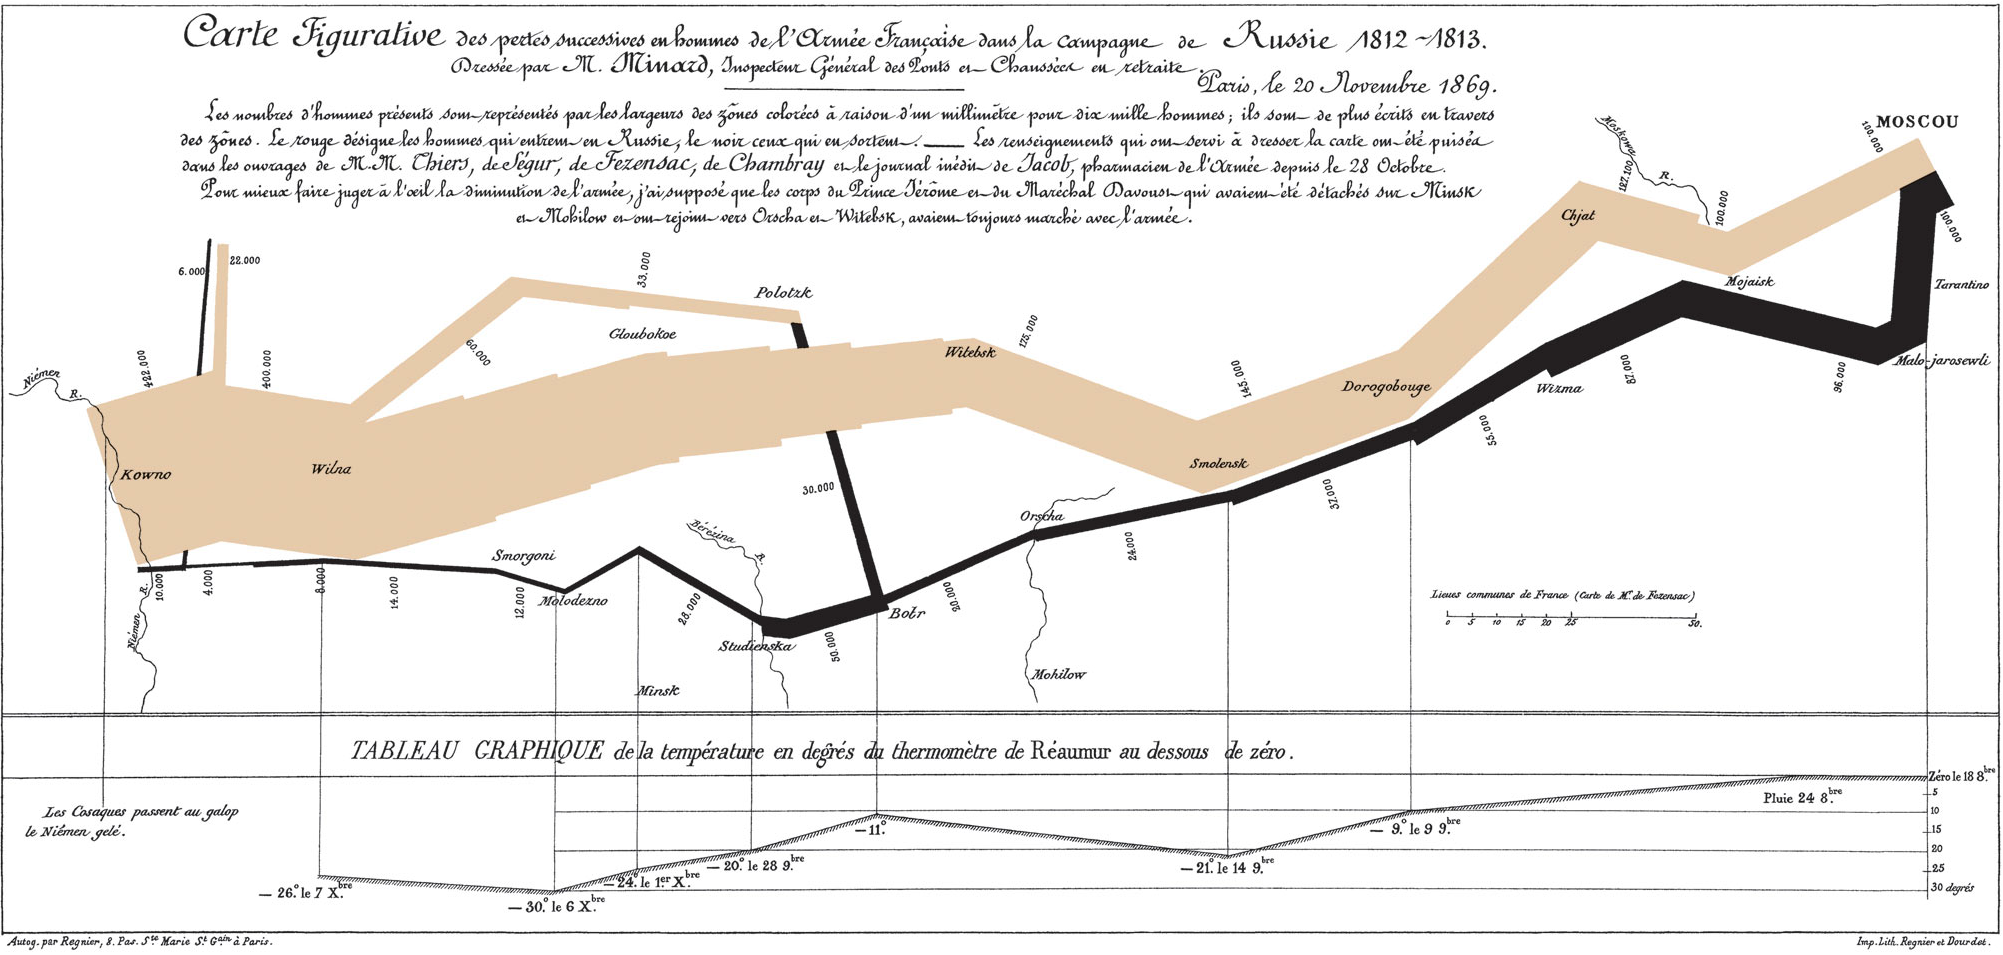
\includegraphics[width = \textwidth]{img/Minard}

\vspace{10pt}

\begin{itemize}\footnotesize
  \item How many variables and what's the unit of observation?
  \begin{itemize}
    \item[Extra:] What's the causal argument being told here?
    \item[] Could we test it with the data we have?
  \end{itemize}
\end{itemize}

\end{frame}
% ----------------------------------------------------

% ----------------------------------------------------
\begin{frame}
\frametitle{}
\centering

Introduce sampling bias (later develop with DAGs)


\end{frame}
% ----------------------------------------------------


% ----------------------------------------------------
\begin{frame}
\frametitle{Missing data in DAG framework}
\centering

Missing completely at random (MCAR)
Missing at random (MAR)
Missing not at random (MNAR)

\end{frame}
% ----------------------------------------------------

\section{Describing variables and relationships}


% ----------------------------------------------------
\begin{frame}
\frametitle{Describing variables}
\centering

\begin{itemize}
  \item What is a \textbf{variable}?
  \item Types?
  \begin{itemize}
    \item<2-> Continuous
    \item<3-> Count
    \item<4-> Ordinal
    \item<5-> Categorical (binary)
    \item<6-> Qualitative (* are really a variable?)
  \end{itemize}
  \item<7-> Why does it matter?
  \item<7-> Conceptual meaning vs statistical meaning
\end{itemize}

\end{frame}
% ----------------------------------------------------

% ----------------------------------------------------
\begin{frame}
\frametitle{Describing variables}
\centering

main idea: variable distribution (of values)

you probably know this because of basic statistics. it doesn't matter so much

kurtosis, normality, blah blah

but one thing though: values are real-world observations. do \textbf{plot} it, and make sure it's coherent with the \textbf{theoretical} or \textbf{expected distribution}

maybe also important: mean +/- SD, or 25/75 percentiles. for effect sizes

in a normal distribution, there not much to say. but e.g. if an independent variable is a bimodal distribution, does that say something about the causal mechanism?

e.g. think about the effect of income on X, in a super unequal society vs one in which is normally distributed

\end{frame}
% ----------------------------------------------------

% ----------------------------------------------------
\begin{frame}
\frametitle{Describing relationships}
\centering

\begin{itemize}
  \item What is a \textbf{relationship}?
  \item Essentially that as you know about the values of one variable, you learn about the values of the other variables
  \item[] e.g. a \textit{negative} relationship means that you know that higher values in $x$ imply lower values in $y$
  \item[]
  \item[]<2-> Imagine you have a small car, and a friend of yours is coming and is bringing along his two kids. Concerned about space, you ask `\textit{how old are they?}` And the answer is: `\textit{They're 6 and 2}.`
  \begin{itemize}
    \item What do you imagine about size?
    \item<3-> Now imagine you ask `\textit{are they blonde, red-haired, or brown-haired?}'
  \end{itemize}
\end{itemize}

\end{frame}
% ----------------------------------------------------

% ----------------------------------------------------
\begin{frame}
\frametitle{Statistical relationship $\neq$ causal relationships}
\centering

\begin{itemize}
  \item<1-> Last example: Is there a causal relationship \textit{age} \rightarrow \textit{size}?
  \item<2-> What if the variable you want to guess is \textbf{the time of the day}, and someone tells you that she just heard the rooster crow? Causal?
  \item[]
  \item<3-> Why are non-causal descriptive relationships \textbf{useful}?
\end{itemize}

\end{frame}
% ----------------------------------------------------

% ----------------------------------------------------
\begin{frame}
\frametitle{Describing relationships}
\centering

conditional distributions
conditional means
conditional conditional means (controlling)

\end{frame}
% ----------------------------------------------------


\section{Example: Wartime civilian deaths}

% ----------------------------------------------------
\begin{frame}
\frametitle{Practical example}
\centering

\begin{itemize}
  \item You want to test an argument about \textbf{wartime civilian deaths:}
  \begin{itemize}
    \item The intuition you have is that civilians will be more likely to be treated well (and not killed) by rebel groups during civil wars when they need their resources (e.g. labor) to survive
  \end{itemize}
  \item[]
  \item Clean up the theory, decide on the main concepts
  \item Develop different RQ at different levels
  \item How can we measure the main concepts? Variables?
  \item What answers could we get from the data?
    \begin{itemize}
      \item Are we learning something about our theory?
    \end{itemize}
\end{itemize}

\end{frame}
% ----------------------------------------------------


%\appendix
%\renewcommand{\theframenumber}{A\arabic{framenumber}}
%\renewcommand{\insertframenumber}{A\arabic{framenumber}}

% ====================================================
\end{document}
